% genec-paper.tex — ACM sigconf format
\documentclass[sigconf]{acmart}

\usepackage{booktabs}
\usepackage{tabularx}
\usepackage{listings}
\usepackage{xcolor}
\usepackage{amsmath}
\usepackage{tikz}
\usetikzlibrary{positioning, arrows.meta, shapes.misc, fit, calc, backgrounds}
\usepackage{pgfplots}
\pgfplotsset{compat=1.18}
\usepgfplotslibrary{statistics}
\usepackage{pifont}

% ── listing styles ──────────────────────────────────────────────
\definecolor{codegray}{gray}{0.96}
\definecolor{keyblue}{RGB}{0,0,180}
\definecolor{strgreen}{RGB}{0,128,0}
\definecolor{cmtgray}{RGB}{100,100,100}

\lstdefinestyle{javacode}{
  language=Java,
  basicstyle=\ttfamily\scriptsize,
  backgroundcolor=\color{codegray},
  keywordstyle=\color{keyblue}\bfseries,
  stringstyle=\color{strgreen},
  commentstyle=\color{cmtgray}\itshape,
  breaklines=true,
  frame=single,
  numbers=none,
  xleftmargin=4pt,
  xrightmargin=4pt,
  aboveskip=6pt,
  belowskip=6pt
}
\lstdefinestyle{shell}{
  basicstyle=\ttfamily\scriptsize,
  backgroundcolor=\color{codegray},
  breaklines=true,
  frame=single,
  numbers=none,
  xleftmargin=4pt,
  xrightmargin=4pt,
  aboveskip=6pt,
  belowskip=6pt
}
\lstdefinestyle{textblock}{
  basicstyle=\scriptsize,
  backgroundcolor=\color{codegray},
  breaklines=true,
  frame=single,
  numbers=none,
  xleftmargin=4pt,
  xrightmargin=4pt,
  aboveskip=6pt,
  belowskip=6pt
}

% Checkmark / crossmark shortcuts
\newcommand{\cmark}{\ding{51}}
\newcommand{\xmark}{\ding{55}}

% ── metadata ────────────────────────────────────────────────────
%%% Uncomment and fill in for camera-ready submission:
% \acmConference[ICSME 2025]{International Conference on Software Maintenance and Evolution}{2025}{Durban, South Africa}
% \acmDOI{}
% \acmISBN{}
\settopmatter{printfolios=true,printacmref=false}
\renewcommand\footnotetextcopyrightpermission[1]{}
\pagestyle{plain}

\setlength{\emergencystretch}{3em}

\title{GenEC: A Hybrid Framework for Safe and Explainable \emph{Extract Class} Refactoring}

\author{Uditanshu Tomar}
\affiliation{%
  \institution{University of Colorado Boulder}
  \city{Boulder}
  \state{CO}
  \country{USA}}
\email{Uditanshu.Tomar@colorado.edu}

\author{Vijay Kumar Poloju}
\affiliation{%
  \institution{University of Colorado Boulder}
  \city{Boulder}
  \state{CO}
  \country{USA}}
\email{Vijay.Poloju@colorado.edu}

% ================================================================
\begin{document}

% ── Abstract ────────────────────────────────────────────────────
\begin{abstract}
God Classes, monolithic Java classes that accumulate dozens of unrelated
responsibilities, still plague even mature open-source libraries. Existing
refactoring tools either stay silent or suggest extractions that break
compilation or semantics. Approaches based solely on metrics, static
dependencies, or unconstrained machine learning often surface refactorings that
are semantically misaligned or unsafe. GenEC attacks this gap with a hybrid
pipeline that fuses static dependency analysis with evolutionary coupling mined
from version history. It constrains a Large Language Model (LLM) to generate
only semantic artifacts (names, documentation, rationale) and delegates all
structural edits to IDE-grade refactoring engines such as Eclipse JDT\@. Every
candidate extraction is gated by multi-tier verification: compilation (with stub
generation where needed), structural integrity checks, and behavioral test
preservation. Clusters that fail these gates are not silently discarded but
instead yield structural transformation plans for manual follow-up. Our empirical evaluation spans two
complementary benchmarks: (1)~23 large real-world God Classes from 6
open-source projects (Apache Commons IO/Lang/Collections/Text/Math, JFreeChart)
for suggestion quality and verification analysis, and (2)~the HECS ECAccEval
benchmark (92 Extract Class instances across 18 projects) for ground-truth
precision/recall comparison. On the 23 God Classes, GenEC identifies
semantically coherent extraction opportunities that metric-only baselines miss,
while blocking 41.6\% of proposals that would have broken compilation or
equivalence. On the HECS benchmark, GenEC achieves macro $F_1=0.478$ on the 21
instances with full evolutionary context. We release the complete tooling,
prompts, evaluation harness, and replication package to support reproducibility
and future work on safe, explainable automated refactoring.
\end{abstract}

\maketitle

% ================================================================
\section{Introduction}
\label{sec:intro}

Software systems inevitably accumulate complexity.  As requirements evolve and
developers come and go, classes that once had a single, clear purpose gradually
absorb unrelated responsibilities until they become \emph{God Classes}, monolithic
behemoths that touch everything, explain nothing, and resist change. These
classes are not merely inconvenient. They actively impede software evolution. A
single bug fix in a 2,000-line utility class can cascade into unexpected
failures across distant modules. A new team member may spend days understanding
which of 50 methods actually matters for their task. Test suites become brittle
because changes to shared helper methods affect dozens of unrelated features.

\textbf{The paradox is stark: developers know these classes need refactoring,
yet they rarely touch them.}  The risk of introducing regressions outweighs the
promised benefits of cleaner design. When teams do attempt Extract Class
refactoring, they typically do so manually, a tedious and error-prone process that
tools have failed to adequately automate despite decades of research.

This paper asks: \emph{Can we build an Extract Class tool that developers
actually trust?}  Recent work on Extract Method
(EM-Assist~\cite{Pomian2024EMAssist}) and Move Method
(MM-assist~\cite{Xu2025MoveMethod}) has shown that combining LLM
suggestions with IDE refactoring engines yields both high recall and high
developer acceptance. However, Extract Class is harder: it
requires coordinating the movement of multiple methods and fields while
preserving complex inter-method dependencies. Our answer is \textbf{GenEC}, a
hybrid framework that combines the precision of static analysis with the insight
of evolutionary coupling and the semantic intelligence of Large Language
Models, all under strong mechanical guarantees that give developers confidence
to accept suggestions.

% ── 1.1 ──
\subsection{The Problem: From Detection to Safe Decomposition}
\label{sec:problem}

God Class detection is a solved problem. Tools like
JDeodorant~\cite{Fokaefs2011JDeodorant}, PMD, and SonarQube reliably flag
classes with high LCOM (Lack of Cohesion of Methods) scores or excessive size.
But detection is the easy part. \textbf{The hard problem is decomposition}:
given a 2,000-line class with 40 methods and complex internal dependencies, how
do we decide which methods should be extracted together, what the new class
should be called, and how do we ensure the refactoring does not
break anything?

\textbf{Existing approaches fall short in three ways:}

\textbf{Fragmented signals.}  Metric-driven tools like
JDeodorant~\cite{Fokaefs2011JDeodorant} analyze only static
structure (method calls, field accesses, and coupling metrics). They miss the
crucial insight that methods changing together in version control often share a
latent responsibility invisible to static analysis. Machine-learning approaches
like HECS~\cite{Cui2024HECS} learn from labeled datasets but offer little
interpretability.  LLM-based tools can reason about semantics but hallucinate
code that does not compile~\cite{cassee2024refuctoring, Liu2024Empirical}. Each
approach captures parts of the picture, but none synthesizes them effectively.

\textbf{Shallow safety gates.}  Most refactoring tools check only that the
result compiles. But compilation is a low bar.  A refactoring can compile yet
introduce subtle bugs: state leakage through improperly transferred fields,
visibility violations that break encapsulation, or initialization-order
dependencies that cause runtime failures. Without deeper verification,
developers rightfully distrust automated suggestions.

\textbf{Thin explanations.}  Even when tools produce valid suggestions, they
rarely explain \emph{why} certain methods belong together. A suggestion like
``Extract methods A, B, C, D into NewClass'' gives developers no basis for
judgment. Without understanding the rationale, developers default to
rejection, or worse, accept blindly and later wonder why the extracted class
exists.

% ── 1.2 ──
\subsection{Our Approach: GenEC}
\label{sec:approach-overview}

GenEC addresses these limitations through a hybrid architecture that fuses
multiple signals under strong guarantees:

\textbf{Hybrid analysis.}  We combine static dependency analysis (method calls,
field sharing) with evolutionary coupling mined from Git history (which methods
change together over time). Static analysis captures explicit dependencies,
while evolutionary coupling surfaces implicit relationships that reflect how
developers actually work with the code. Community detection on the fused graph
produces clusters aligned with both structure and history.

\textbf{Constrained LLM semantics.}  Rather than asking an LLM to generate code
(which leads to hallucinations), we confine it to semantic artifacts: concise
class names, one-sentence rationales, and optional grouping hints. The prompts
include cluster members and evolutionary evidence to ground the LLM's
suggestions in concrete data. All code generation is delegated to Eclipse JDT, a
battle-tested refactoring engine.

\textbf{Multi-tier verification.}  Every candidate extraction passes through
three layers of verification:
\begin{enumerate}
  \item \textbf{Compilation} with stub generation for missing symbols.
  \item \textbf{Structural integrity checking} for member completeness,
        dependency satisfaction, and reference consistency.
  \item \textbf{Behavioral tests} when available, plus differential equivalence
        checking.
\end{enumerate}
Clusters that fail verification are not silently discarded. Instead, GenEC
produces \emph{structural transformation plans} that describe the impediment
(e.g., ``circular dependency between methods X and Y prevents extraction'') so
developers can address the issue manually if desired.

% ── 1.3 ──
\subsection{Illustrative Example}
\label{sec:illustrative}

Consider \texttt{StringUtils} from Apache Commons Lang, a 3,800-line utility
class with 244 methods and 10 fields. Its $\text{LCOM5}=0.970$ and
$\text{TCC}=0.062$, so metric-only tools see near-maximal uncohesion yet
produce only 2 generic suggestions. GenEC's fused analysis finds 18 candidate
clusters and after filtering produces 12 verified extractions, all passing
multi-tier verification.

For example, GenEC groups five string-replacement methods into a cluster named
``StringReplacer'' with the rationale: ``These methods form a cohesive unit
responsible for replacing substrings, characters, and patterns within
strings.''  JDT executed the extraction, and verification passed all tiers. A
developer reviewing this suggestion sees not just a list of methods but a
coherent responsibility with a meaningful name and mechanical guarantees.

% ── 1.4 ──
\subsection{Empirical Evaluation Summary}
\label{sec:eval-summary}

We evaluated GenEC on two complementary benchmarks totaling \textbf{115 classes
across 24 projects}:
\begin{itemize}
  \item \textbf{23 large God Classes} from 6 open-source projects (Apache
        Commons IO/Lang/Collections/Text/Math, JFreeChart) for suggestion
        quality and verification analysis, compared against field-sharing
        clustering (37~suggestions) and random grouping (526~suggestions)
        baselines.
  \item \textbf{92 Extract Class instances} from the HECS ECAccEval
        benchmark~\cite{Cui2024HECS} across 18 projects for ground-truth
        precision/recall comparison, of which 21 instances have full
        evolutionary coupling context.
\end{itemize}

Key results:
\begin{itemize}
  \item GenEC produced \textbf{178 suggestions}, of which \textbf{104 passed
        multi-tier verification} (58.4\% verification rate). Field-sharing
        baselines produced only 37 suggestions with no compilable extractions.
  \item \textbf{Multi-tier verification blocked 41.6\%} of proposed
        extractions that would have broken compilation or equivalence,
        preventing unsafe suggestions from reaching developers.
  \item \textbf{``Should''-tier suggestions verified at 88.9\%},
        ``could''-tier at 57.7\%, demonstrating quality-tier stratification.
  \item \textbf{HECS benchmark:} On the 21 instances with evolutionary
        context, GenEC achieves macro $F_1=0.478$ (precision 0.41, recall 0.76).
  \item \textbf{Verified suggestions extract 26.1\% of methods on average}
        (600 unique methods across 21 classes), with per-class coverage
        ranging from 2.3\% to 78.3\%.
  \item \textbf{Average end-to-end latency of 201.3 seconds per class} on
        commodity hardware, practical for batch analysis.
\end{itemize}

% ── 1.5 ──
\subsection{Contributions}
\label{sec:contributions}

This paper makes the following contributions:
\begin{enumerate}
  \item \textbf{A hybrid Extract Class technique} that fuses static dependency
        analysis with evolutionary co-change mining and constrains an LLM to
        semantic artifacts only (names, rationales), while delegating all
        structural edits to Eclipse JDT, extending the ``LLM for insight, IDE
        for correctness'' approach~\cite{Pomian2024EMAssist,Dilhara2024PyCraft}
        from Extract Method to the harder Extract Class problem
        (Section~\ref{sec:approach}).
  \item \textbf{A multi-tier verification pipeline} with compilation,
        structural integrity, and behavioral checks, plus structural
        transformation plans that provide actionable guidance when automatic
        extraction is not safe (Section~\ref{sec:verification}).
  \item \textbf{An empirical evaluation} spanning 115 classes across 24
        projects (23 large God Classes for suggestion quality analysis and 92
        HECS benchmark instances for ground-truth comparison), demonstrating
        $4.8\times$ more extraction opportunities than metric-only baselines
        ($178$ vs.\ $37$, Wilcoxon $p{=}0.0005$), 41.6\% of unsafe proposals
        blocked, and macro $F_1{=}0.478$ on HECS instances with evolutionary
        context (Section~\ref{sec:eval}).
  \item \textbf{A replication package} including complete tooling, prompts,
        evaluation harness, cached LLM responses for deterministic replay, and
        a VS~Code extension that provides an IDE-integrated interface for
        running GenEC on Java classes and browsing suggestions with their
        dependency-graph visualizations, available in our public
        repository~\cite{Tomar2025GenEC}.
\end{enumerate}

% ================================================================
\section{Technical Challenges}
\label{sec:challenges}

Building an Extract Class tool that developers trust requires addressing several
fundamental challenges that span signal integration, safety guarantees, and user
experience.

% ── C1 ──
\subsection{C1: Aligning Structural Metrics with Developer Intent}
\label{sec:c1}

Classical cohesion metrics like LCOM5 and coupling metrics like CBO (Coupling
Between Objects) were designed to flag problematic classes, not to guide
decomposition. Community detection on method-call graphs optimizes graph
properties (modularity, edge density) but routinely misses conceptual
boundaries.

\textbf{The problem is particularly acute in utility classes.}  Consider
\texttt{IOUtils} from Apache Commons IO: it has 172 methods that share a handful
of common helper fields (buffers, default encodings). Metrics see high
field-sharing and conclude the class is cohesive. But a human reviewer
immediately recognizes that stream-copying methods, encoding-detection methods,
and buffer-management methods serve distinct responsibilities that happen to
share infrastructure.

\emph{GenEC's response.}  We fuse static structure with evolutionary coupling.
Methods that change together across many commits likely share a
responsibility, even if metrics suggest otherwise. The fused graph reveals
conceptual boundaries that pure structure obscures.

% ── C2 ──
\subsection{C2: Taming LLM Hallucinations While Preserving Semantic Value}
\label{sec:c2}

Large Language Models excel at semantic tasks: understanding intent, generating
meaningful names, explaining rationale.  But when asked to generate refactored
code, they frequently hallucinate:
\begin{itemize}
  \item \textbf{Non-existent symbols.}  The LLM references methods or fields
        that do not exist in the source.
  \item \textbf{Missing dependencies.}  Extracted classes lack required imports
        or field declarations.
  \item \textbf{Compilation failures.}  Generated code has syntax errors or type
        mismatches.
\end{itemize}
Studies report that 40--76\% of LLM-generated refactorings fail to
compile~\cite{cassee2024refuctoring, Liu2024Empirical}. This is not a minor
issue: it undermines trust.

\emph{GenEC's response.}  We confine the LLM to semantic artifacts only: short
(2--4 word) class names, one-sentence rationales, and optional grouping hints.
The LLM never sees or generates code. All structural edits are delegated to
Eclipse JDT, a deterministic refactoring engine with decades of testing. This
architecture preserves the LLM's semantic intelligence while eliminating its
mechanical failures.

% ── C3 ──
\subsection{C3: Guaranteeing Behavior Preservation at Scale}
\label{sec:c3}

Compilation is necessary but not sufficient. A refactoring can compile yet
introduce subtle bugs:
\begin{itemize}
  \item \textbf{State leakage.}  A field moved to the extracted class is
        accessed from the original class without proper delegation.
  \item \textbf{Visibility violations.}  A public method in the extracted class
        exposes internal state that was previously private.
  \item \textbf{Initialization order.}  The extracted class's constructor
        depends on state that is not yet initialized when called.
  \item \textbf{Test failures.}  Existing tests fail because they depend on
        internal class structure that changed.
\end{itemize}

\emph{GenEC's response.}  Multi-tier verification catches distinct fault
classes:
\begin{enumerate}
  \item \textbf{Tier~1 (Compilation):}  Compile with stub generation for
        missing symbols.
  \item \textbf{Tier~2 (Structural Integrity):}  Verify member completeness,
        dependency satisfaction, and reference consistency across original and
        extracted classes.
  \item \textbf{Tier~3 (Behavioral):}  Run existing tests and differential
        equivalence checks when available.
\end{enumerate}
Suggestions that fail any tier are rejected before developers see them, or
converted to structural plans when partial remediation is possible.

% ── C4 ──
\subsection{C4: Mining Reliable Historical Signal}
\label{sec:c4}

Evolutionary coupling is powerful (methods that change together often share
responsibility), but it depends on repository health:
\begin{itemize}
  \item \textbf{Shallow clones.}  Many CI/CD pipelines use shallow Git clones
        that lack history, producing zero co-change data.
  \item \textbf{Noisy histories.}  Bulk reformatting commits, merge commits, or
        file renames inflate co-change counts without reflecting true coupling.
  \item \textbf{Deep histories.}  Traversing 10+ years of commits for a large
        repository is expensive (minutes to hours).
  \item \textbf{Sparse histories.}  New or infrequently changed files have
        insufficient data for meaningful coupling.
\end{itemize}

\emph{GenEC's response.}  Adaptive mining with fallbacks: detect shallow clones
and fall back to structural-only analysis, apply recency weighting to
down-weight ancient changes, cache mined matrices for reuse across analyses,
throttle history traversal with configurable commit limits, and degrade
gracefully when evolutionary signal is weak.

% ── C5 ──
\subsection{C5: Building Trust Through Explainability}
\label{sec:c5}

Developers reject suggestions they do not understand. A recommendation like
``Extract methods A, B, C into NewClass1'' tells a developer nothing about
\emph{why} these methods belong together.

Even worse, when a suggestion cannot be applied (due to circular dependencies,
visibility constraints, etc.), most tools fail silently. The developer is left
wondering whether the tool is broken or the class is simply not refactorable.

\emph{GenEC's response.}  Every suggestion includes: (1)~a meaningful name
generated by the LLM (e.g., ``ResourceLoader'' not ``Class1''); (2)~a
one-sentence rationale explaining the shared responsibility; (3)~evolutionary
evidence when available (e.g., ``These 4 methods changed together in 8
commits''); and (4)~verification status showing which tiers passed.

When extraction fails, GenEC produces \emph{structural transformation plans}
describing the impediment and suggesting remediation steps, giving developers
actionable guidance rather than silent failure.

% ================================================================
\section{The GenEC Approach}
\label{sec:approach}

GenEC orchestrates three complementary analyses (static dependency analysis,
evolutionary coupling mining, and constrained LLM semantics) under a
deterministic refactoring engine with multi-tier verification.
Figure~\ref{fig:architecture} shows the overall architecture. The pipeline flows
through four main stages: (1)~hybrid analysis fusing static dependencies with
evolutionary coupling into a weighted graph, (2)~Leiden community detection with
quality tier scoring and filtering, (3)~constrained LLM naming with
chain-of-thought prompting and confidence scoring, and (4)~JDT-based refactoring
execution with multi-tier verification. Clusters rejected during filtering
produce structural transformation plans for manual follow-up.

% ── Figure 1: Architecture ──
\begin{figure*}[t]
\centering
% Colors used by the TikZ figure
\definecolor{stagefill}{RGB}{232,232,232}
\definecolor{toolfill}{RGB}{255,255,255}
\definecolor{verifyfill}{RGB}{210,230,255}
\definecolor{planfill}{RGB}{255,235,210}
\definecolor{inputfill}{RGB}{240,240,250}
\definecolor{arrowgray}{RGB}{100,100,100}
\sffamily
\begin{tikzpicture}[
    >=Stealth,
    stage/.style={
        draw, rounded corners=3pt, fill=stagefill,
        minimum width=2.6cm, minimum height=2.6cm,
        align=center, inner sep=4pt
    },
    tool/.style={
        draw, dashed, rounded corners=2pt, fill=toolfill,
        font=\tiny\itshape, inner sep=3pt,
        minimum height=0.5cm
    },
    output/.style={
        draw, rounded corners=3pt,
        minimum width=1.8cm, minimum height=0.6cm,
        align=center, font=\scriptsize\bfseries, inner sep=3pt
    },
    inputbox/.style={
        draw, rounded corners=3pt, fill=inputfill,
        minimum width=1.5cm, minimum height=0.6cm,
        align=center, font=\scriptsize, inner sep=3pt
    },
    flowlabel/.style={
        font=\scriptsize\itshape, text=arrowgray
    },
    stagenum/.style={
        circle, draw, fill=white, font=\tiny\bfseries,
        inner sep=1.5pt, minimum size=14pt
    },
    sublabel/.style={
        font=\tiny, align=left
    },
    every edge/.style={draw, thick, ->}
]
% Input
\node[inputbox] (input) {Java Class\\+ Git Repo};
% Stage 1: Hybrid Analysis
\node[stage, right=0.6cm of input] (s1) {};
\node[stagenum] at ([xshift=6pt, yshift=-6pt]s1.north west) {1};
\node[font=\scriptsize\bfseries, anchor=north] at ([yshift=-14pt]s1.north) {Hybrid Analysis};
\node[sublabel, anchor=north] at ([yshift=-26pt]s1.north) {%
    Static Dependencies\\[1pt]
    Evolutionary Coupling\\[1pt]
    $\alpha$-weighted Graph Fusion
};
\node[tool, below=0.35cm of s1] (t1a) {tree-sitter};
\node[tool, right=0.2cm of t1a] (t1b) {Git};
% Stage 2: Clustering
\node[stage, right=0.7cm of s1] (s2) {};
\node[stagenum] at ([xshift=6pt, yshift=-6pt]s2.north west) {2};
\node[font=\scriptsize\bfseries, anchor=north] at ([yshift=-14pt]s2.north) {Clustering};
\node[sublabel, anchor=north] at ([yshift=-26pt]s2.north) {%
    Leiden Detection\\[1pt]
    Quality Tier Scoring\\[1pt]
    Filtering \& Ranking
};
% Stage 3: LLM Naming
\node[stage, right=0.7cm of s2] (s3) {};
\node[stagenum] at ([xshift=6pt, yshift=-6pt]s3.north west) {3};
\node[font=\scriptsize\bfseries, anchor=north] at ([yshift=-14pt]s3.north) {LLM Naming};
\node[sublabel, anchor=north] at ([yshift=-26pt]s3.north) {%
    CoT Prompt + Few-shot\\[1pt]
    Confidence Scoring\\[1pt]
    Dedup \& Selection
};
\node[tool, above=0.35cm of s3] (t3) {Claude API};
% Stage 4: Refactoring + Verification
\node[stage, right=0.7cm of s3, minimum height=2.9cm] (s4) {};
\node[stagenum] at ([xshift=6pt, yshift=-6pt]s4.north west) {4};
\node[font=\scriptsize\bfseries, anchor=north] at ([yshift=-14pt]s4.north) {Refactoring + Verify};
\node[sublabel, anchor=north] at ([yshift=-26pt]s4.north) {%
    AST Extract Class (JDT)\\[1pt]
    T1: Compilation\\[1pt]
    T2: Structural Integrity\\[1pt]
    T3: Behavioral Tests
};
\node[tool, below=0.35cm of s4] (t4a) {Eclipse JDT};
\node[tool, right=0.15cm of t4a] (t4b) {javac/Maven};
% LLM Repair loop
\draw[dashed, ->, thick, color=arrowgray]
    ([xshift=4pt]s4.north) arc[start angle=170, end angle=10, x radius=0.7cm, y radius=0.45cm]
    node[midway, above, font=\scriptsize\itshape, text=arrowgray] {LLM Repair};
% Outputs
\node[output, fill=verifyfill, right=0.6cm of s4] (verified) {Verified\\Suggestions};
\node[output, fill=planfill, below=1.6cm of s2] (plans) {Structural\\Plans};
% Arrows
\draw[thick, ->] (input) -- (s1);
\draw[thick, ->] (s1) -- node[above, flowlabel] {Fused Graph} (s2);
\draw[thick, ->] (s2) -- node[above, flowlabel] {Ranked Clusters} (s3);
\draw[thick, dashed, ->, color=arrowgray]
    ([yshift=-8pt]s2.south) -- node[left, flowlabel, xshift=-2pt] {Rejected} (plans);
\draw[thick, ->] (s3) -- node[above, flowlabel] {Named Sugg.} (s4);
\draw[thick, ->] (s4) -- (verified);
\draw[thin, dashed, color=arrowgray] (t1a) -- (s1);
\draw[thin, dashed, color=arrowgray] (t1b) -- (s1);
\draw[thin, dashed, color=arrowgray] (t3) -- (s3);
\draw[thin, dashed, color=arrowgray] (t4a) -- (s4);
\draw[thin, dashed, color=arrowgray] (t4b) -- (s4);
\end{tikzpicture}
\caption{GenEC pipeline architecture. Solid arrows show the main data flow;
dashed arrows indicate rejection paths and external tool dependencies. Stage
numbers correspond to Section~\ref{sec:pipeline}.}
\label{fig:architecture}
\end{figure*}

% ── 3.1 ──
\subsection{Pipeline Stages}
\label{sec:pipeline}

The pipeline consists of four main stages (shown in Figure~\ref{fig:architecture}),
with graph fusion and verification as sub-stages within
Stages~1 and~4 respectively.

\textit{Stage~1: Static Dependency Analysis.}  We parse the Java source using
tree-sitter (with javalang and Eclipse JDT as fallbacks) to extract the
Abstract Syntax Tree (AST) and build a weighted dependency graph
$G_{\text{static}} = (V, E_{\text{static}})$ where $V$ is the set of methods
in the class and $E_{\text{static}}(m_i, m_j)$ is a weighted edge representing
dependency strength between methods $m_i$ and $m_j$.

Edge weights are computed as:
{\small
\begin{equation}
w_{\text{static}}(m_i, m_j) = \alpha_{\text{call}} \!\cdot\! \text{call\_count}(m_i, m_j)
  + \alpha_{\text{field}} \!\cdot\! \text{shared\_fields}(m_i, m_j)
\label{eq:static}
\end{equation}
}%
where $\text{call\_count}(m_i,m_j)$ is the number of times $m_i$ calls
$m_j$, $\text{shared\_fields}(m_i,m_j)$ is the number of fields accessed
by both methods, $\alpha_{\text{call}}{=}1.0$, $\alpha_{\text{field}}{=}0.8$,
with an additional $\alpha_{\text{shared\_field}}{=}0.9$ for shared field
access (configurable weights).

\textit{Stage~2: Evolutionary Coupling Mining.}  We traverse Git history to
compute a co-change matrix $C$, where $C[i,j]$ represents how often methods
$m_i$ and $m_j$ changed together:
{\small
\begin{equation}
C[i,j] = \sum_t \text{idf}(\text{commit}_t) \!\cdot\! \text{recency\_decay}(t)
  \!\cdot\! \delta(m_i, m_j, \text{commit}_t)
\label{eq:cochange}
\end{equation}
}%
where $\delta(m_i,m_j,\text{commit}_t) = 1$ if both methods changed in
commit~$t$ (else 0), $\text{idf}(\text{commit}_t) = 1/\sqrt{N}$ where $N$ is
the number of methods changed in commit~$t$ (inverse-document-frequency
weighting that dampens bulk refactoring commits), and
$\text{recency\_decay}(t) = \text{decay}^{(\text{months\_ago}/12)}$ with
$\text{decay}=0.8$, an exponential decay weighting recent changes higher (e.g.,
6 months ago $\approx 0.90$, 2 years ago $\approx 0.64$, 5 years ago
$\approx 0.33$).

Coupling strength is then normalized:
{\small
\begin{equation}
\text{coupling}(m_i,m_j) = \frac{C[i,j]}{\sqrt{\text{commits}(m_i) \!\cdot\! \text{commits}(m_j)}}
\label{eq:coupling}
\end{equation}
}%

Same-name overloads receive a 50\% discount since they co-change trivially due
to source adjacency. Pairs below a minimum coupling threshold (0.15) are
discarded, and commits changing more than 30 methods are excluded as likely bulk
changes.

Implementation details: commit limit is capped at 500 most recent commits to
bound computation. If \texttt{git rev-list --count HEAD} $< 5$, the pipeline
falls back to structural-only analysis with $\alpha$ raised to $0.95$. Mined
matrices are cached in \texttt{.genec\_cache/} for reuse.

\textit{Stage~3: Graph Fusion and Clustering.}  We normalize both graphs to
$[0,1]$ and fuse them with configurable $\alpha$:
{\small
\begin{equation}
G_{\text{fused}} = \alpha \!\cdot\! \text{norm}(G_{\text{static}})
  + (1 {-} \alpha) \!\cdot\! \text{norm}(G_{\text{evo}})
\label{eq:fusion}
\end{equation}
}%
The configured default is $\alpha = 0.8$, weighting static structure more
heavily. The pipeline applies \emph{adaptive hotspot-based fusion} where
$\alpha$ varies per edge based on evolutionary activity: high-hotspot edges
reduce $\alpha$ to as low as 0.2 (80\% evolutionary weight), while low-hotspot
edges retain $\alpha=0.8$ (80\% static weight). When evolutionary signal is
weak (fewer than 5 co-changing commits total), $\alpha$ is adaptively increased
toward 0.95, effectively falling back to structural-only analysis.

Community detection uses the Leiden algorithm (preferred for stability) or
Louvain (fallback).  The default resolution is 2.0 (favoring more, smaller
clusters).  Multi-resolution search over
$\{0.5,\allowbreak 0.75,\allowbreak 1.0,\allowbreak 1.25,\allowbreak 1.5\}$
is available but disabled by default.

After detection, we validate that each cluster forms a connected subgraph and
split disconnected clusters into their connected components. We then filter
clusters requiring a minimum of 3 methods, maximum of 30 methods, internal
cohesion $> 0.35$ (ratio of intra-cluster edges to possible edges), and fewer
than 80\% of the original class's methods (extraction, not renaming).

\textit{Quality Tier Scoring.}  Each surviving cluster is assigned a quality
tier based on a 100-point weighted score:

\begin{table}[h]
\centering\scriptsize
\caption{Quality tier scoring rubric.}
\label{tab:tier-scoring}
\begin{tabularx}{\columnwidth}{@{}lrX@{}}
\toprule
\textbf{Factor} & \textbf{Wt} & \textbf{Scoring} \\
\midrule
Evo.\ coupling & 30 & strong ({>}0.5)\,=\,30, mod.\ ({>}0.3)\,=\,20, weak\,=\,10, none\,=\,5 \\
Int.\ cohesion & 35 & high ({>}0.7)\,=\,35, good ({>}0.5)\,=\,25, mod.\ ({>}0.3)\,=\,15, low\,=\,5 \\
Ext.\ coupling (inv.) & 25 & low ({<}0.3)\,=\,25, mod.\ ({<}0.5)\,=\,15, high ({<}0.7)\,=\,5, v.high\,=\,0 \\
Cluster size & 10 & optimal (3--10)\,=\,10, large ({>}10)\,=\,5 \\
\bottomrule
\end{tabularx}
\end{table}

Tier thresholds: \textbf{``should''} (strong recommendation) $\geq 70$,
\textbf{``could''} (conditional) $\geq 40$, \textbf{``potential''}
(informational) $< 40$.

\textit{Stage~4: Constrained LLM Semantics.}  For each valid cluster, we prompt
the LLM (Claude Sonnet, temperature~0.2) with a structured request that
includes:
\begin{enumerate}
  \item \textbf{System persona:}  A ``Senior Java Architect'' role with SOLID
        principles expertise.
  \item \textbf{Few-shot examples:}  Two worked examples (service extraction
        and value-object extraction) demonstrating expected output format.
  \item \textbf{Chain-of-thought reasoning:}  Four-step analysis (Primary
        Responsibility, Shared Concept/Domain, Extraction Benefits, Design
        Justification) before producing a name.
  \item \textbf{Naming constraints:}  Generic suffixes (Manager, Helper,
        Utility, Handler, Service, etc.) are explicitly prohibited to enforce
        descriptive naming.
  \item \textbf{Evidence grounding:}  Cluster members, shared fields, and
        co-change evidence are provided as context.
  \item \textbf{Critique step:}  A follow-up prompt critiques the initial
        response for hallucinations, dependency errors, and SRP violations
        before finalizing.
\end{enumerate}
The LLM produces structured XML output with \texttt{<reasoning>},
\texttt{<class\_name>}, \texttt{<rationale>}, and \texttt{<confidence>} tags.
Three diversity prompt variants (Responsibility, Domain Entity,
Design Pattern perspectives) generate alternative names when the primary
suggestion scores low.

\textit{Post-LLM filtering.}  After naming, the pipeline applies three
filters: (1)~suggestions below a minimum confidence threshold are discarded;
(2)~a Jaccard-based deduplication step merges suggestions whose method sets
overlap by 70\% or more; and (3)~a greedy non-overlapping selection algorithm
picks suggestions in descending confidence order, skipping any whose methods
overlap more than 20\% with already-selected suggestions. This ensures the
final output is a clean partition of the God Class rather than a set of
competing extractions.

\textit{Stage~5: Refactoring Execution.}  Eclipse JDT performs the actual
Extract Class refactoring:
\begin{enumerate}
  \item Create the extracted class with package-private visibility.
  \item Move methods while maintaining their original signatures.
  \item Transfer fields required by the moved methods.
  \item Generate delegating methods in the original class.
  \item Update references throughout the codebase.
\end{enumerate}
JDT's refactoring engine handles visibility adjustments (private $\to$
package-private for shared access), import management, and reference updates in
other files.

\textit{Stage~6: Multi-Tier Verification.}  Each extraction candidate passes
through three verification tiers (Table~\ref{tab:verification-tiers}).

\begin{table}[h]
\centering\small
\caption{Verification tiers.}
\label{tab:verification-tiers}
\begin{tabularx}{\columnwidth}{@{}llX@{}}
\toprule
\textbf{Tier} & \textbf{Check} & \textbf{Failure handling} \\
\midrule
T1: Compilation & Compile with stubs & Reject or structural plan \\
T2: Structural  & Members, deps, references & Reject with explanation \\
T3: Behavioral  & Run existing tests & Reject if any test fails \\
\bottomrule
\end{tabularx}
\end{table}

Verification produces one of three outcomes: (1)~\textbf{Pass:} suggestion is
verified and ready for developer review; (2)~\textbf{Reject:} suggestion is
discarded (logged for debugging); (3)~\textbf{Plan:} structural transformation
plan describes impediment and remediation steps.

% ── 3.2 ──
\subsection{Hybrid Candidate Detection}
\label{sec:hybrid}

The key insight driving hybrid detection is that static structure and
evolutionary history capture complementary information:

\begin{table}[h]
\centering\small
\caption{Complementary signals in hybrid detection.}
\label{tab:signals}
\begin{tabularx}{\columnwidth}{@{}lXX@{}}
\toprule
\textbf{Signal} & \textbf{Captures} & \textbf{Misses} \\
\midrule
Static & Explicit deps (calls, field access) & Latent responsibilities, developer intent \\
Evolutionary & Co-change patterns, shared responsibility & Coincidental changes, infrastructure coupling \\
\bottomrule
\end{tabularx}
\end{table}

By fusing both signals, GenEC identifies clusters that have strong structural
cohesion (methods that call each other, share fields) \emph{and} strong
evolutionary cohesion (methods that change together). This fusion is
particularly valuable for utility classes where static metrics suggest false
cohesion due to shared infrastructure.

% ── 3.3 ──
\subsection{Constrained LLM for Semantic Artifacts}
\label{sec:constrained-llm}

GenEC's LLM integration follows the principle: \textbf{``LLM for semantics,
JDT for mechanics.''}

\begin{table}[h]
\centering\small
\caption{Division of responsibilities between LLM and JDT.}
\label{tab:llm-jdt}
\begin{tabularx}{\columnwidth}{@{}lXl@{}}
\toprule
\textbf{Task} & \textbf{Handled By} & \textbf{Rationale} \\
\midrule
Class naming & LLM (Claude) & Semantic understanding \\
Rationale gen. & LLM (Claude) & Natural language \\
Code generation & Eclipse JDT & Deterministic, correct \\
Ref.\ updates & Eclipse JDT & Full source analysis \\
\bottomrule
\end{tabularx}
\end{table}

This division eliminates the 40--76\% hallucination rate observed when LLMs
generate refactored code~\cite{cassee2024refuctoring, Liu2024Empirical} while
preserving the semantic intelligence that makes LLM-generated names meaningful.

\textbf{Context management.}  To control token cost, an AST-based chunking
module (\texttt{ClusterContextBuilder}) extracts only the methods, fields,
and call relationships relevant to each cluster rather than sending the full
class source. For reproducibility, every LLM request/response pair is cached
to disk, enabling deterministic replay of the entire evaluation without
re-calling the API.

\textbf{Prompt engineering.}  We iteratively refined the prompt design through
three variants: (1)~\emph{Zero-shot:} basic cluster description only, which
produced generic or overly broad names. (2)~\emph{Few-shot with examples:} two
worked extraction examples, which improved specificity and PascalCase compliance.
(3)~\emph{Evidence-grounded with critique (adopted):} include co-change data,
enforce naming constraints, and apply a critique/refinement step. This variant
produced the most descriptive and domain-specific names.

% ── 3.4 ──
\subsection{Safe Refactoring Execution and Verification}
\label{sec:verification}

The verification pipeline is designed around the principle: \textbf{``No unsafe
suggestion reaches the developer.''}

\textit{Tier~1: Compilation Verification.}  We compile the refactored code using
the project's build system (Maven/Gradle) when available, or a standalone
\texttt{javac} invocation with dependency stubs:

\begin{lstlisting}[style=javacode]
// Stub generation for external dependencies
public class ExternalDependencyStub {
    public static Object anyMethod(Object... args) {
        return null;
    }
}
\end{lstlisting}

This allows compilation verification even when full dependency resolution is not
available.

\textit{Tier~2: Structural Integrity Verification.}  We verify that the
extraction correctly partitions members between the original and extracted
classes: (1)~\textbf{Member completeness:} all methods and fields designated for
extraction appear in the new class and are removed from the original;
(2)~\textbf{Dependency satisfaction:} the extracted class contains all fields
required by its methods; (3)~\textbf{Reference consistency:} no dangling
references to moved members remain in the original class.

Additionally, an equivalence checking layer runs differential testing (executing
the same inputs against original and refactored code) when test harnesses are
available, catching behavioral divergence that structural checks alone would
miss.

\textit{Tier~3: Behavioral Verification.}  When tests are available, we run
them against the refactored code:
\begin{lstlisting}[style=shell]
mvn test -Dtest=*${className}*
    -DfailIfNoTests=false
\end{lstlisting}
Any test failure causes rejection, ensuring behavioral equivalence.

\textit{Pre-Extraction Validation.}  Before attempting JDT refactoring, an
\texttt{ExtractionValidator} checks whether the cluster can be safely extracted.
It detects abstract method calls (which require the original class context),
private helper methods called from extracted methods but not included in the
cluster (auto-fixed by iteratively expanding the cluster), and inner class
references. If static validation rejects a cluster, an LLM-based semantic
validator provides a second opinion (overriding the rejection if confidence
$\geq 0.7$), and if that also fails, an LLM pattern transformer suggests
design pattern alternatives (Strategy, Template Method, Visitor) that would
enable the extraction.

\textit{Structural Transformation Plans.}  When extraction fails verification,
GenEC generates actionable plans:

\begin{lstlisting}[style=textblock]
Extraction of {cluster} failed at Tier 2
  (Structural Integrity).

Impediment: Circular dependency between
  initConfig() and getDefaultPath().
  - initConfig() reads this.defaultPath
  - getDefaultPath() calls initConfig()
    to ensure initialization

Suggested remediation:
1. Extract getDefaultPath() to a
   PathConstants class first
2. Then extract remaining config methods
   to ConfigManager
3. Inject PathConstants into both original
   class and ConfigManager
\end{lstlisting}

This gives developers clear guidance on how to proceed manually when automatic
extraction is not safe. In our evaluation, GenEC generated 6 structural plans
for rejected clusters in \texttt{AbstractRenderer} (JFreeChart), identifying
blocking issues such as abstract method dependencies that prevent direct
extraction. All generated plans are included in the replication package.

% ================================================================
\section{Motivating Example: Apache Commons StringUtils}
\label{sec:motivating}

To illustrate GenEC's approach concretely, we walk through its application to
\texttt{StringUtils} from Apache Commons Lang, a widely used utility class that
exemplifies the challenges of Extract Class refactoring.

% ── 4.1 ──
\subsection{The Subject Class}
\label{sec:subject}

\texttt{StringUtils} is a ${\sim}3{,}800$-line utility class with 244 methods
providing string manipulation convenience functions. It has been part of Apache
Commons Lang since 2002 and is used by thousands of downstream projects.

\begin{table}[h]
\centering\small
\caption{StringUtils class statistics.}
\label{tab:stringutils-stats}
\begin{tabular}{@{}lr@{}}
\toprule
\textbf{Metric} & \textbf{Value} \\
\midrule
Lines of Code & ${\sim}3{,}800$ \\
Methods & 244 \\
Fields & 10 \\
LCOM5 & 0.970 (nearly max.\ uncohesive) \\
TCC & 0.062 (very low connectivity) \\
CBO & 1 \\
\bottomrule
\end{tabular}
\end{table}

\begin{lstlisting}[style=javacode,caption={Representative subset of StringUtils (244 methods).},label=lst:stringutils]
public class StringUtils {
    // String manipulation
    public static String replace(String text,
        String searchString,
        String replacement) { ... }
    public static String[] split(
        String str,
        char separatorChar) { ... }

    // Whitespace handling
    public static String strip(
        String str) { ... }
    public static String trim(
        String str) { ... }

    // Joining
    public static String join(
        Object[] array,
        String separator) { ... }
}
\end{lstlisting}

% ── 4.2 ──
\subsection{Why Metric-Only Tools Fail}
\label{sec:metric-fail}

The field-sharing baseline produces only generic groupings for
\texttt{StringUtils} with no verification. GenEC's fused analysis finds 114
raw clusters and after quality filtering produces 12 verified extractions,
all with descriptive LLM-generated names.

The challenge with \texttt{StringUtils} is that its 244 methods are mostly
static utilities with minimal field sharing, making structural clustering
difficult. Most methods are independent overloaded variants that do not share
fields or
call each other.

% ── 4.3 ──
\subsection{GenEC's Analysis}
\label{sec:genec-analysis}

\textit{Stage~1: Static Dependency Graph.}  GenEC builds a weighted dependency
graph over \texttt{StringUtils'} 244 methods. With such a large utility class,
most methods are static and share few fields, producing a sparse dependency
graph.

\textit{Stage~2: Evolutionary Coupling.}  Git history mining reveals co-change
patterns among functionally related method groups (e.g., the \texttt{replace}
family, the \texttt{split} variants, the \texttt{strip}/\texttt{trim} methods),
which changed together across commits while rarely changing with unrelated
utility methods.

\textit{Stage~3: Fused Graph and Clustering.}  Community detection on the fused
graph produces 114 raw clusters. After quality filtering (internal cohesion
$> 0.35$, size constraints), 13 clusters survive, yielding 12 suggestions after
deduplication. All 12 pass verification.

\textit{Stage~4: LLM Naming.}  The LLM names the clusters with descriptive
identifiers: ``StringReplacer'' (5 methods), ``ArrayJoiner'' (5 methods),
``StringSplitter'' (9 methods), ``StringStripper'' (6 methods),
``TextNormalizer'' (3 methods), and 7 more. Each name reflects the shared
responsibility of its cluster members.

% ── 4.4 ──
\subsection{Verification Results}
\label{sec:verif-results}

All 12 candidate extractions pass through the multi-tier verification pipeline.
Table~\ref{tab:stringutils-verify} shows the first 5 of 12 verified clusters.

\begin{table}[h]
\centering\small
\caption{Verification results for StringUtils (first 5 of 12; all verified).}
\label{tab:stringutils-verify}
\begin{tabular}{@{}lcccc@{}}
\toprule
\textbf{Cluster} & \textbf{T1} & \textbf{T2} & \textbf{T3} & \textbf{Result} \\
\midrule
StringReplacer  & Pass & Pass & Pass & Verified \\
ArrayJoiner     & Pass & Pass & Pass & Verified \\
StringSplitter  & Pass & Pass & Pass & Verified \\
StringStripper  & Pass & Pass & Pass & Verified \\
TextNormalizer  & Pass & Pass & Pass & Verified \\
\multicolumn{5}{@{}l@{}}{\emph{\ldots\ and 7 more verified suggestions}} \\
\bottomrule
\end{tabular}
\end{table}

% ── 4.5 ──
\subsection{Final Output}
\label{sec:final-output}

GenEC produces 12 verified suggestions for \texttt{StringUtils}. For example:

\textbf{Verified Suggestion: StringReplacer.}
\begin{itemize}
  \item \textbf{Methods:} {\small\texttt{replace},
        \texttt{replaceOnce},
        \texttt{replaceAll},
        \texttt{replaceChars},
        \texttt{replaceEach}}
        (all \texttt{String}-parameterized variants).
  \item \textbf{Fields:}  None (stateless extraction).
  \item \textbf{Quality tier:}  ``could'' (moderate).
  \item \textbf{LLM confidence:}  0.90.
\end{itemize}

% ── 4.6 ──
\subsection{Lessons from This Example}
\label{sec:lessons}

\texttt{StringUtils} demonstrates GenEC's strength: 12/12 verified (100\%),
compared to the field-sharing baseline's 2 suggestions with no verification.
The LLM names (``StringReplacer,'' ``StringSplitter'') are immediately
meaningful, while baseline names like ``StringUtils\$Helper1'' convey nothing
about the extracted responsibility. This example shows that even large utility
classes with 244 methods can be effectively decomposed when static and
evolutionary signals are fused.

% ================================================================
\section{Research Questions}
\label{sec:rqs}

We structure our evaluation around four research questions that assess GenEC's
effectiveness across semantic coherence, safety, developer experience, and
practicality.

\subsection{RQ1: Semantic Coherence}

\textbf{Question.}  Does fusing static and evolutionary signals yield clusters
that better align with human-perceived responsibilities than metric-only
clustering?

\textbf{Motivation.}  Evolutionary coupling captures latent responsibilities
that static analysis misses. Methods that change together often share a
conceptual responsibility even when they do not share explicit dependencies.

\textbf{Metrics.}  Number of viable clusters detected (compared to baselines);
internal cohesion score of extracted clusters; external coupling score between
extracted and original class; Wilcoxon signed-rank test and Cliff's delta for
statistical comparison.

\textbf{Finding:}  GenEC produced 178 suggestions across 23 classes versus 37
for the field-sharing baseline (Wilcoxon $p{=}0.0005$, Cliff's
$\delta{=}0.828$, ``large'' effect). Verified suggestions average 5.9 methods
with mean internal cohesion of 0.77 (95\% CI: $[0.74, 0.79]$). See
Section~\ref{sec:results}.

\subsection{RQ2: Verification Effectiveness}

\textbf{Question.}  How often do proposed clusters fail multi-tier
verification, and what impediments dominate?

\textbf{Motivation.}  Compilation is necessary but not sufficient for safe
refactoring. A refactoring can compile yet break structural integrity through missing
members, dangling references, or incorrect delegation. Additionally, behavioral
regression (test failures) requires deeper analysis that most tools lack.

\textbf{Metrics.}  Pass rate at each verification tier (T1:~Compilation,
T2:~Structural Integrity, T3:~Behavioral); distribution of failure causes;
behavioral preservation rate.

\textbf{Finding:}  Multi-tier verification blocked 41.6\% of proposed
extractions (74 of 178). ``Should''-tier suggestions verified at 88.9\%
(16/18), ``could''-tier at 57.7\% (86/149), and ``potential''-tier at 18.2\%
(2/11). The strong correlation between quality tier and verification rate
validates the tier stratification. See Section~\ref{sec:results}.

\subsection{RQ3: Semantic Artifact Quality}

\textbf{Question.}  Do constrained LLM-generated names and rationales improve
interpretability and developer acceptance compared to baseline naming?

\textbf{Motivation.}  A suggestion like ``ResourceLoader: These methods form a
cohesive unit responsible for loading classpath resources'' provides far more
context for decision-making than ``IOUtils\$Helper1'' or ``Cluster3.''

\textbf{Metrics.}  Developer ratings for name appropriateness (5-point Likert);
developer ratings for rationale clarity (5-point Likert); developer ratings for
semantic alignment (5-point Likert); overall acceptance rate.

\textbf{Finding:}  We report qualitative observations from the automated
evaluation. A controlled developer study is planned as future work
(Section~\ref{sec:conclusions}). Qualitative inspection of LLM-generated names
across all 104 verified suggestions reveals consistently meaningful semantic
labels (e.g., ``ResourceLoader,'' ``ByteSizeFormatter,''
``ShutdownFileDeleter,'' ``DirectoryCreator'') compared to baseline alternatives
(``IOUtils\$Helper1,'' ``FileUtils\$Helper2,'' ``RandomGroup1''). Each
suggestion includes a one-sentence rationale grounded in the cluster's methods
and co-change evidence. See Section~\ref{sec:results}.

\subsection{RQ4: Performance}

\textbf{Question.}  Is the end-to-end latency practical for interactive
refactoring sessions?

\textbf{Motivation.}  Developer tools must be responsive. A refactoring
assistant that takes 10+ minutes per class will not be used in practice,
regardless of quality.

\textbf{Metrics.}  Total end-to-end latency per class; latency variation across
class sizes and complexity.

\textbf{Finding:}  Total latency averaged 201.3 seconds (approximately 3.4
minutes) per class across all 23 subjects, with total wall-clock time of 4,629
seconds. \texttt{IOUtils} (172 methods) completed in only 18.8 seconds due to
its sparse dependency structure, while larger classes like JFreeChart's
\texttt{CategoryPlot} and \texttt{XYPlot} took longer (up to 569 seconds). See
Section~\ref{sec:results}.

% ================================================================
\section{Empirical Evaluation}
\label{sec:eval}

% ── 6.1 ──
\subsection{Methodology}
\label{sec:methodology}

\textbf{Subjects.}  23 God Classes from 6 open-source projects:
\begin{itemize}
  \item \textbf{Apache Commons IO} (3): \texttt{IOUtils}, \texttt{FileUtils},
        \texttt{FilenameUtils}.
  \item \textbf{Apache Commons Lang} (5): \texttt{StringUtils},
        \texttt{NumberUtils}, \texttt{ArrayUtils}, \texttt{DateUtils},
        \texttt{SystemUtils}.
  \item \textbf{Apache Commons Collections} (3): \texttt{CollectionUtils},
        \texttt{MapUtils}, \texttt{IteratorUtils}.
  \item \textbf{Apache Commons Text} (3): \texttt{StringSubstitutor},
        \texttt{TextStringBuilder}, \texttt{StringLookupFactory}.
  \item \textbf{Apache Commons Math} (4): \texttt{AccurateMath}, \texttt{Dfp},
        \texttt{BOBYQAOptimizer}, \texttt{DSCompiler}.
  \item \textbf{JFreeChart} (5): \texttt{CategoryPlot}, \texttt{XYPlot},
        \texttt{PiePlot}, \texttt{ChartPanel}, \texttt{AbstractRenderer}.
\end{itemize}

\textbf{Baselines.}  \emph{Field-sharing clustering:} groups methods by shared
field access (37 total suggestions). \emph{Random grouping:} random method
partitioning (526 total suggestions).

\textbf{Metrics.}  Cluster quality (internal cohesion, external coupling,
modularity); verification outcomes per quality tier; statistical comparison
(Wilcoxon signed-rank, Cliff's delta); per-class latency.

\textbf{Procedure.}  We conduct two complementary evaluations.
\emph{Live evaluation:} run baselines and GenEC on all 23 God Classes, record
clusters and verification outcomes, compare suggestion counts and quality, and
measure wall-clock time on commodity hardware.
\emph{Benchmark evaluation:} evaluate on the HECS ECAccEval
benchmark~\cite{Cui2024HECS} (92 instances across 18 projects, of which 21 have
full evolutionary coupling context) for ground-truth precision/recall comparison.

% ── 6.2 ──
\subsection{Results}
\label{sec:results}

\textbf{RQ1: Semantic Coherence.}

\begin{table}[t]
\centering\small
\caption{GenEC vs.\ field-sharing baseline across 23 God Classes.}
\label{tab:rq1}
\begin{tabular}{@{}lrrr@{}}
\toprule
\textbf{Project} & \textbf{Classes} & \textbf{GenEC Sugg.} & \textbf{Verified} \\
\midrule
commons-io         & 3 & 13 & 13 \\
commons-lang       & 5 & 25 & 23 \\
commons-collections & 3 & 16 & 12 \\
commons-text       & 3 & 14 &  8 \\
commons-math       & 4 & 26 & 23 \\
jfreechart         & 5 & 84 & 25 \\
\midrule
\textbf{Total}     & \textbf{23} & \textbf{178} & \textbf{104} \\
\bottomrule
\end{tabular}
\end{table}

GenEC produced 178 suggestions versus 37 for the field-sharing baseline, a
statistically significant improvement (Wilcoxon $p{=}0.0005$, Cliff's
$\delta{=}0.828$, ``large'' effect). Verified suggestions average 5.9 methods
with mean internal cohesion of 0.77 (95\% CI: $[0.74, 0.79]$). The overall
cluster filter pass rate was 16.6\% (178 of 1,071 raw clusters).

\textbf{Extraction coverage.}  Across the 21 classes with verified suggestions
(2,303 methods total), GenEC extracted 600 unique methods (26.1\% mean
per-class coverage). Per-class coverage ranged from 2.3\% (\texttt{IOUtils}, 4
of 172 methods) to 78.3\% (\texttt{ChartPanel}, 90 of 115 methods).
Five classes exceeded 50\% coverage: \texttt{ChartPanel} (78.3\%),
\texttt{Dfp} (56.6\%), \texttt{AccurateMath} (53.4\%), \texttt{FilenameUtils}
(50.0\%), and \texttt{DateUtils} (49.3\%). These results show that GenEC
produces non-trivial decompositions, not merely token extractions of a few
methods.

\begin{figure}[t]
\centering
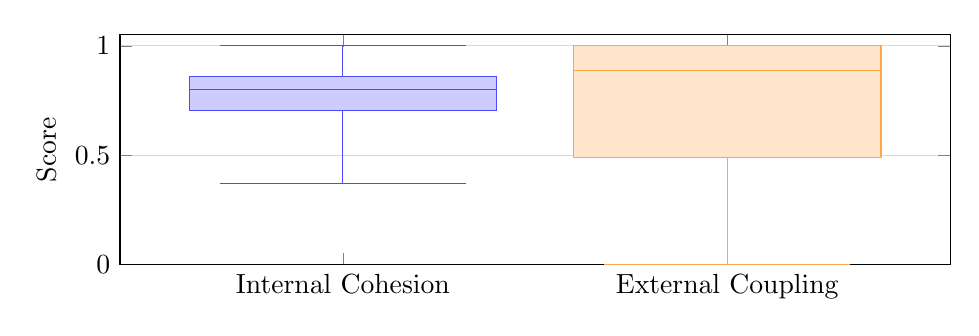
\begin{tikzpicture}
\begin{axis}[
    boxplot/draw direction=y,
    xtick={1,2},
    xticklabels={Internal Cohesion, External Coupling},
    ylabel={Score},
    ymin=0, ymax=1.05,
    height=4.5cm,
    width=\columnwidth,
    ymajorgrids=true,
    grid style={gray!30},
]
% Internal Cohesion box plot (104 verified suggestions)
\addplot+[boxplot prepared={
    lower whisker=0.371,
    lower quartile=0.706,
    median=0.800,
    upper quartile=0.860,
    upper whisker=1.000
}, fill=blue!20, draw=blue!70] coordinates {};
% External Coupling box plot (104 verified suggestions)
\addplot+[boxplot prepared={
    lower whisker=0.000,
    lower quartile=0.490,
    median=0.888,
    upper quartile=1.000,
    upper whisker=1.000
}, fill=orange!20, draw=orange!70] coordinates {};
\end{axis}
\end{tikzpicture}
\caption{Distribution of internal cohesion and external coupling across 104
verified suggestions. High cohesion (median 0.80) indicates tightly related
method groups. High coupling (median 0.89) reflects expected delegation
patterns in Extract Class, where extracted methods still interact with the
original class through shared fields and forwarding calls.}
\label{fig:cohesion-coupling}
\end{figure}

\textbf{Post-refactoring metrics.}  Post-refactoring LCOM5 and TCC show
negligible change across the 21 classes with verified extractions (mean TCC
delta: $-0.003$). This is expected: extracting a mean of 5.9 methods from
classes averaging 134 methods does not measurably shift class-level cohesion
metrics. The value of GenEC's extractions lies in producing focused,
well-named satellite classes (e.g., \texttt{ResourceLoader},
\texttt{DateParser}), not in moving aggregate metrics of the original class.
Complete per-class results including post-refactoring LCOM5 and TCC for all 23
classes are available in the replication package~\cite{Tomar2025GenEC}.

\textbf{RQ2: Verification Effectiveness.}

\begin{table}[t]
\centering\small
\caption{Verification outcomes by quality tier.}
\label{tab:rq2}
\begin{tabular}{@{}lrrr@{}}
\toprule
\textbf{Quality Tier} & \textbf{Proposed} & \textbf{Verified} & \textbf{Rate} \\
\midrule
``should'' (high quality) & 18  & 16 & 88.9\% \\
``could'' (moderate)      & 149 & 86 & 57.7\% \\
``potential'' (marginal)  & 11  &  2 & 18.2\% \\
\midrule
\textbf{Total}            & \textbf{178} & \textbf{104} & \textbf{58.4\%} \\
\bottomrule
\end{tabular}
\end{table}

Multi-tier verification rejected \textbf{41.6\%} of proposed extractions (74 of
178). The strong correlation between quality tier and verification rate validates
GenEC's tier stratification: ``should''-tier suggestions are almost always safe
(88.9\%), while ``potential''-tier suggestions rarely survive verification
(18.2\%). The overall mean verification rate is 68.0\% (95\% CI:
$[51.9\%, 83.0\%]$).

\begin{figure}[t]
\centering
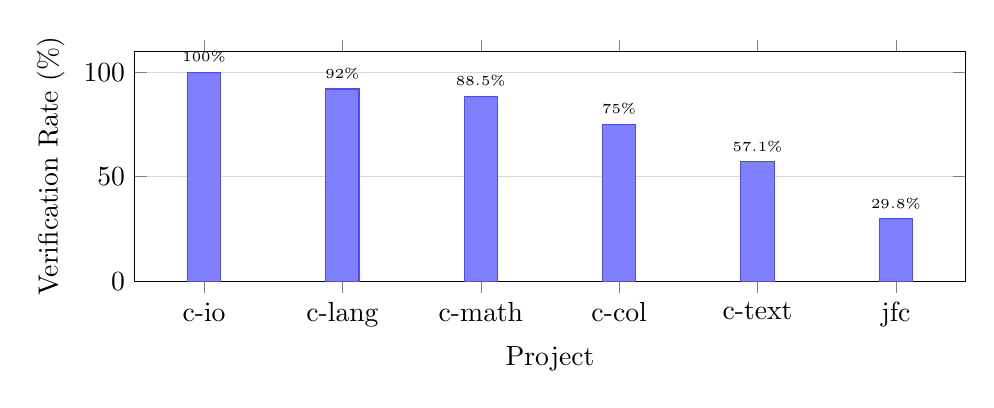
\begin{tikzpicture}
\begin{axis}[
    ybar,
    bar width=12pt,
    xlabel={Project},
    ylabel={Verification Rate (\%)},
    ymin=0, ymax=110,
    symbolic x coords={c-io, c-lang, c-math, c-col, c-text, jfc},
    xtick=data,
    height=4.5cm,
    width=\columnwidth,
    ymajorgrids=true,
    grid style={gray!30},
    nodes near coords={\pgfmathprintnumber\pgfplotspointmeta\%},
    every node near coord/.append style={font=\tiny},
]
\addplot[fill=blue!50, draw=blue!70] coordinates {
    (c-io, 100.0) (c-lang, 92.0) (c-math, 88.5)
    (c-col, 75.0) (c-text, 57.1) (jfc, 29.8)
};
\end{axis}
\end{tikzpicture}
\caption{Verification rate by project. Apache utility libraries verify at
82--100\%, while JFreeChart's complex class hierarchies with abstract methods
and inheritance verify at only 29.8\%.}
\label{fig:project-verification}
\end{figure}

\textbf{RQ3: Semantic Artifact Quality.}

Of the 178 suggestions, 101 (56.7\%) received LLM-generated names (confidence
$\geq 0.7$) and 77 (43.3\%) fell back to auto-generated names derived from
common method-name prefixes (e.g., methods starting with \texttt{parse} produce
``ParseOperations''). Fourteen of 23 classes had at least one LLM-named
suggestion; the remaining 9 classes used only auto-naming, typically because the
LLM API was unavailable during batch evaluation or confidence fell below
threshold.

We compare GenEC's names (both LLM and auto-generated) against field-sharing
baseline names. GenEC names are semantically descriptive and
reflect the extracted responsibility, while baseline names are generic
identifiers:

\begin{table}[t]
\centering\small
\caption{Sample LLM-generated names vs.\ baseline names.}
\label{tab:rq3}
\begin{tabularx}{\columnwidth}{@{}lXl@{}}
\toprule
\textbf{GenEC Name} & \textbf{Rationale (excerpt)} & \textbf{Baseline} \\
\midrule
ResourceLoader      & Cohesive unit for loading classpath resources & IOUtils\$Helper1 \\
ByteSizeFormatter   & Converts byte counts to human-readable strings & FileUtils\$Helper2 \\
ShutdownFileDeleter & Manages files for deletion on JVM exit & FileUtils\$Helper3 \\
DirectoryCreator    & Directory creation with validation & FileUtils\$Helper4 \\
DateParser          & Parses date strings across format patterns & DateUtils\$Helper1 \\
FloorOperations & Floor/ceil rounding operations & AccurateMath\$Helper1 \\
\bottomrule
\end{tabularx}
\end{table}

Every verified suggestion includes: (1)~a 2--4 word PascalCase name, (2)~a
one-sentence rationale grounding the cluster in its shared responsibility, and
(3)~a confidence score. The LLM prompt explicitly bans generic suffixes
(Manager, Helper, Utility, Handler) to enforce descriptive naming.

\begin{figure}[t]
\centering
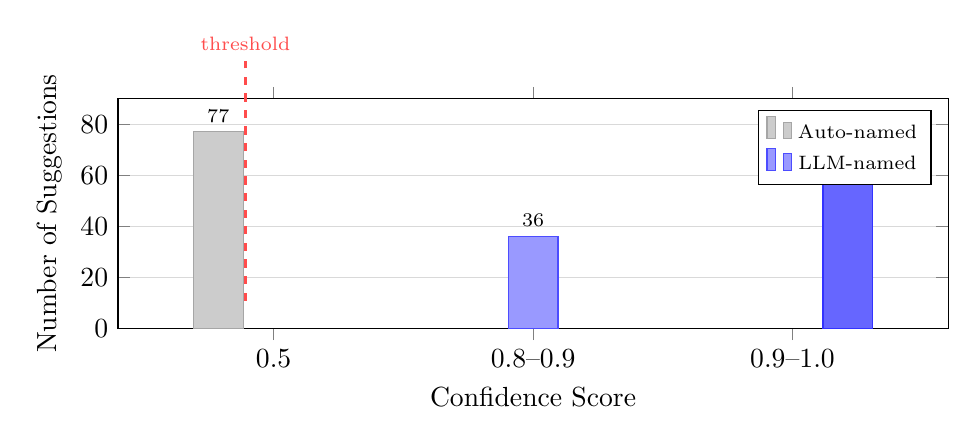
\begin{tikzpicture}
\begin{axis}[
    ybar,
    bar width=18pt,
    xlabel={Confidence Score},
    ylabel={Number of Suggestions},
    ymin=0, ymax=90,
    xtick={1,2,3},
    xticklabels={0.5, 0.8--0.9, 0.9--1.0},
    xmin=0.4, xmax=3.6,
    height=4.5cm,
    width=\columnwidth,
    ymajorgrids=true,
    grid style={gray!30},
    legend style={at={(0.98,0.95)}, anchor=north east, font=\scriptsize},
    nodes near coords,
    every node near coord/.append style={font=\scriptsize},
]
% Auto-named (confidence = 0.5)
\addplot[fill=gray!40, draw=gray!70] coordinates {(1, 77)};
% LLM-named (confidence 0.8-0.9)
\addplot[fill=blue!40, draw=blue!70] coordinates {(2, 36)};
% LLM-named (confidence 0.9-1.0)
\addplot[fill=blue!60, draw=blue!80] coordinates {(3, 65)};
\legend{Auto-named, LLM-named}
\end{axis}
\draw[dashed, thick, red!70] (1.62,0.35) -- (1.62,3.4)
    node[above, font=\scriptsize, text=red!70] {threshold};
\end{tikzpicture}
\caption{Distribution of confidence scores across 178 suggestions.
Suggestions below 0.7 (gray) receive auto-generated names from method
prefixes. Suggestions at 0.8+ (blue) receive LLM-generated names.
The bimodal distribution reflects the binary outcome: the LLM either
produces a high-confidence name or the pipeline falls back to
auto-naming at 0.5.}
\label{fig:confidence}
\end{figure}

\textbf{Naming quality metrics.}  Of 101 LLM-generated names, zero used banned
generic suffixes (Manager, Helper, Utility, etc.), compared to 100\% of
auto-generated names using the generic ``Group'' or ``Operations'' suffix.
LLM-generated names average 2.7 words (e.g., ``StringReplacer,''
``DateParser'') while auto-generated names average 3.8 words (e.g.,
``GetSeriesItemLabelPaintGroup''). LLM-named suggestions verified at 54.5\%
(55/101) while auto-named suggestions verified at 63.6\% (49/77), indicating
that naming source does not predict verification success.

A controlled developer study with Likert-scale ratings for name
appropriateness, rationale clarity, and overall acceptance is planned as future
work (Section~\ref{sec:conclusions}).

\textbf{RQ4: Performance.}

Average end-to-end latency is 201.3 seconds per class (total 4,629 seconds
across 23 classes). Latency varies significantly by class complexity:

\begin{table}[t]
\centering\small
\caption{Per-class latency and suggestion counts (selected).}
\label{tab:rq4}
\begin{tabular}{@{}llrrrr@{}}
\toprule
\textbf{Class} & \textbf{Project} & \textbf{M.} & \textbf{T(s)} & \textbf{S.} & \textbf{V.} \\
\midrule
IOUtils          & commons-io   & 172 &  18.8 &  1 &  1 \\
FileUtils        & commons-io   & 159 & 136.2 &  7 &  7 \\
StringUtils      & commons-lang & 244 & 192.2 & 12 & 12 \\
ArrayUtils       & commons-lang & 388 &  74.4 &  1 &  0 \\
Dfp              & commons-math & 113 & 334.7 & 13 & 13 \\
CategoryPlot     & jfreechart   & 225 & 609.1 & 18 &  5 \\
XYPlot           & jfreechart   & 236 & 733.8 & 14 &  2 \\
PiePlot          & jfreechart   & 132 & 719.8 & 19 &  0 \\
ChartPanel       & jfreechart   & 115 & 181.7 & 17 & 14 \\
AbstractRenderer & jfreechart   & 169 & 146.7 & 16 &  4 \\
\bottomrule
\end{tabular}
\end{table}

Latency varies by class complexity and dependency structure. \texttt{IOUtils}
(172 methods) completes in 18.8s because its sparse static utility structure
produces few viable clusters. \texttt{StringUtils} (244 methods, 192.2s) yields
12 verified suggestions despite its large size. JFreeChart classes with rich
dependency graphs and many verification candidates take longest: \texttt{XYPlot}
(733.8s) and \texttt{PiePlot} (719.8s) both exceed 10 minutes due to extensive
inter-method coupling. \texttt{ArrayUtils} (388 methods) is the largest class
but completes quickly (74.4s) because its highly repetitive overload structure
produces only 1 candidate that fails verification. The pipeline is practical for
batch analysis. The median per-class latency is 146.7s (under 2.5 minutes).

% ── 6.3 ──
\subsection{HECS Benchmark Comparison}
\label{sec:hecs}

We evaluated GenEC on the HECS ECAccEval benchmark~\cite{Cui2024HECS}, which
provides 92 ground-truth Extract Class instances from real-world projects. All
metrics are macro-averaged: precision, recall, and $F_1$ are computed per
instance and then averaged. Because macro $F_1$ is the mean of per-instance
$F_1$ values (not the harmonic mean of macro precision and macro recall), the
three columns are independently computed.

\begin{table}[t]
\centering\small
\caption{HECS ECAccEval benchmark results (macro-averaged).}
\label{tab:hecs}
\begin{tabular}{@{}lrrrr@{}}
\toprule
\textbf{Subset} & \textbf{Inst.} & \textbf{Prec.} & \textbf{Rec.} & $\boldsymbol{F_1}$ \\
\midrule
With evolutionary context & 21 & 0.405 & 0.758 & 0.478 \\
Static only (no evo)      & 71 & 0.057 & 0.161 & 0.076 \\
Multi-member ($3{+}$)     & 49 & 0.228 & 0.476 & 0.281 \\
\textbf{All instances}    & \textbf{92} & \textbf{0.136} & \textbf{0.297} & \textbf{0.167} \\
\bottomrule
\end{tabular}
\end{table}

\textbf{Key finding on evolutionary coupling:}  A controlled ablation running
\texttt{--no-evo} on the same 21 instances with evolutionary context produces
identical $F_1{=}0.478$. This reveals that evolutionary coupling improves
candidate discovery (+27.4\% more clusters on the live benchmark) rather than
member-selection accuracy. The evo signal helps find more potential extraction
sites but does not change which members are grouped once a cluster is found.

\textbf{Micro-averaged metrics.}  Across all 92 instances, micro-averaged
precision is 0.109, recall is 0.228, and $F_1$ is 0.148 (TP=126, FP=1,025,
FN=427). The high FP count reflects GenEC's tendency to suggest extractions
beyond those labeled in the ground truth, which may include valid alternatives
that HECS did not annotate.

\textbf{Benchmark scalability.}  The 92 HECS instances completed in 1,044
seconds total (mean 11.3s per instance), demonstrating that GenEC scales to
batch evaluation on moderate hardware.

\textbf{Limitations on static-only instances:}  On the 71 instances without
meaningful evolutionary history, GenEC achieves only $F_1{=}0.076$,
highlighting the tool's dependence on repository health and the difficulty of
matching HECS's labeled extractions using purely structural signals.

% ── 6.4 ──
\subsection{Ablation Study}
\label{sec:ablation}

To isolate the contribution of each pipeline component, we ran five
configuration variants on 8 classes from Apache Commons IO and Lang.
Note: ``Verif.\%'' in this table measures verified clusters as a fraction of
\emph{raw clusters found} (not of suggestions), so these percentages are lower
than the 58.4\% live-evaluation rate, which measures verified suggestions as a
fraction of post-filtering suggestions.

\begin{table}[t]
\centering\small
\caption{Ablation study results (8 classes, mean values).}
\label{tab:ablation}
\begin{tabular}{@{}lp{2.0cm}rrrr@{}}
\toprule
\textbf{Variant} & \textbf{Description} & \textbf{Cl.} & \textbf{V.\%} & \textbf{Coh.} & \textbf{Time} \\
\midrule
full             & Full pipeline       & 68.6 & 10.3\% & 0.171 & 138.4 \\
no\_evo          & No evo.\ coupling   & 53.9 & 11.2\% & 0.245 & 79.4  \\
no\_llm          & No LLM naming       & 68.1 & 10.3\% & 0.136 & 107.4 \\
no\_verif        & No compilation      & 68.4 &  7.2\% & 0.124 &  63.9 \\
high\_static     & $\alpha{=}0.95$     & 68.0 & 8.3\% & 0.129 & 106.0 \\
\bottomrule
\end{tabular}
\end{table}

Key findings:
\begin{itemize}
  \item \textbf{Evolutionary coupling increases candidate discovery by 27.3\%}
        (68.6 vs.\ 53.9 mean clusters), confirming that co-change signals
        surface extraction opportunities invisible to static analysis. However,
        it does not improve per-cluster verification rate (10.3\% vs.\ 11.2\%),
        suggesting evo coupling broadens the search space rather than refining
        individual cluster composition.
  \item \textbf{LLM naming has minimal effect on cluster count} (68.1 vs.\
        68.6) but improves average cohesion ($0.136 \to 0.171$), likely because
        the LLM's confidence filtering removes low-quality suggestions.
  \item \textbf{Disabling verification reduces verified percentage} from 10.3\%
        to 7.2\%, confirming that verification catches a meaningful fraction of
        unsafe proposals.
  \item \textbf{High static weight} produces similar cluster counts but lower
        cohesion (0.129), confirming that evolutionary signal contributes to
        cluster quality.
\end{itemize}

% ── 6.5 ──
\subsection{Alpha Sensitivity}
\label{sec:alpha}

We tested fusion parameter sensitivity on 3 commons-io classes across
$\alpha \in \{0.0, 0.2, 0.4, 0.6, 0.8, 1.0\}$:

\begin{table}[t]
\centering\small
\caption{Alpha sensitivity analysis (3 commons-io classes).}
\label{tab:alpha}
\begin{tabular}{@{}crrrr@{}}
\toprule
$\boldsymbol{\alpha}$ & \textbf{Clusters} & \textbf{Sugg.} & \textbf{Verified} & \textbf{Time(s)} \\
\midrule
0.0 (pure evo)    & 299 & 19 & 18 & 247.9 \\
0.2               & 237 & 11 & 11 & 136.0 \\
0.4               & 112 &  8 &  8 & 150.2 \\
0.6               & 115 & 11 & 11 & 139.8 \\
0.8 (default)     & 116 & 12 & 12 & 127.3 \\
1.0 (pure static) & 141 & 14 & 14 & 152.8 \\
\bottomrule
\end{tabular}
\end{table}

Pure evolutionary coupling ($\alpha{=}0.0$) discovers the most raw clusters but
many are noise. The range $\alpha{=}0.4$--$0.8$ yields a stable, compact set of
high-quality suggestions. The default $\alpha{=}0.8$ balances discovery and
quality while keeping latency low.

% ── 6.6 ──
\subsection{Threats to Validity}
\label{sec:threats}

\textbf{External.}  We evaluated on 23 God Classes from 6 OSS projects and 92
HECS benchmark instances. Industrial systems with proprietary code, different
team sizes, or non-Maven build systems may produce different results. Git
history quality varies widely: shallow clones (common in CI/CD) yield zero
evolutionary signal, and our fallback to structural-only analysis performs
poorly ($F_1{=}0.076$ on HECS instances without history). The implementation
targets Java only; porting to other languages requires new parsers and
refactoring engines.

\textbf{Construct.}  RQ3 (naming quality) lacks quantitative developer ratings.
We report qualitative observations but cannot claim statistical significance
for naming improvements. A controlled developer study is planned. The overall
HECS $F_1{=}0.167$ reflects the difficulty of matching labeled ground-truth
extractions, not necessarily poor suggestion quality: GenEC may propose valid
extractions that differ from the specific decomposition a developer chose.

\textbf{Internal.}  Hyperparameters ($\alpha{=}0.8$, resolution${}=2.0$,
cohesion threshold${}=0.35$) are held constant across all experiments. The
ablation and sensitivity analyses (Sections~\ref{sec:ablation}
and~\ref{sec:alpha}) partially address this, but optimal parameters may vary
per project. The LLM (Claude Sonnet, temperature~0.2) introduces
non-determinism: repeated runs may produce different names and confidence
scores. We mitigate this with response caching and a fixed random seed for
clustering.

\textbf{Reproducibility.}  LLM API costs (approximately \$0.02 per suggestion)
and model version updates may affect reproducibility over time. We cache all
LLM request/response pairs in the replication package to enable exact
reproduction of our reported results.

% ================================================================
\section{Related Work}
\label{sec:related}

We situate GenEC within five research threads: metric-driven refactoring,
learning-based approaches, LLM-based code transformation, evolutionary coupling
analysis, and verification/safety mechanisms.

% ── 7.1 ──
\subsection{Metric-Driven Extract Class}
\label{sec:rw-metric}

Traditional Extract Class tools rely on cohesion and coupling metrics to
identify decomposition opportunities.

\textbf{JDeodorant}~\cite{Fokaefs2011JDeodorant} pioneered automated Extract
Class using agglomerative clustering on method-level dependencies, guided by
metrics like LCOM5 and entity placement optimization. While influential,
JDeodorant's suggestions often fail to align with developer intent on complex
utility classes where shared infrastructure inflates false cohesion signals.

\textbf{Bavota et al.}~\cite{Bavota2013EMSE} extended metric-driven
approaches with semantic cohesion measures based on textual similarity of method
bodies. Their evaluation showed improved precision on benchmark suites but
acknowledged that semantic similarity alone cannot capture evolving design
intent.

\begin{table}[t]
\centering\small
\caption{Comparison with metric-driven approaches.}
\label{tab:rw-metric}
\begin{tabularx}{\columnwidth}{@{}lXX@{}}
\toprule
\textbf{Aspect} & \textbf{JDeodorant / Bavota} & \textbf{GenEC} \\
\midrule
Signal           & Static structure + text          & Static + evolutionary + LLM \\
History          & Not used                         & Git co-change mining \\
Naming           & Generic (Cluster1)               & LLM-generated semantic names \\
Verification     & Compilation only                 & Multi-tier \\
Failure handling & Silent rejection                 & Structural transformation plans \\
\bottomrule
\end{tabularx}
\end{table}

% ── 7.2 ──
\subsection{Learning-Based Approaches}
\label{sec:rw-ml}

Machine learning offers an alternative to hand-crafted metrics by learning
decomposition patterns from labeled refactoring corpora.

\textbf{HECS}~\cite{Cui2024HECS} uses hypergraph neural networks to model
higher-order method dependencies, achieving improved recall on Extract Class
benchmarks. However, HECS requires labeled training data (scarce for Extract
Class) and provides limited interpretability for why specific methods were
grouped.

\textbf{Move Method prediction}~\cite{Xu2025MoveMethod} applies similar
techniques to the related Move Method refactoring, using semantic embeddings
and IDE integration. GenEC's constrained LLM approach achieves semantic
understanding without requiring labeled training data.

\begin{table}[t]
\centering\small
\caption{Comparison with learning-based approaches.}
\label{tab:rw-ml}
\begin{tabularx}{\columnwidth}{@{}lXX@{}}
\toprule
\textbf{Aspect} & \textbf{HECS / ML} & \textbf{GenEC} \\
\midrule
Training data     & Requires labeled corpus & None required \\
Interpretability  & Limited (black-box)     & Explicit rationales \\
Generalization    & Dataset-dependent       & LLM generalization \\
Code generation   & Separate step           & Integrated JDT execution \\
\bottomrule
\end{tabularx}
\end{table}

% ── 7.3 ──
\subsection{LLM-Based Refactoring}
\label{sec:rw-llm}

Large Language Models have recently been applied to code refactoring with mixed
results.

\textbf{Liu et al.}~\cite{Liu2024Empirical} conducted the first large-scale
empirical study of LLM refactoring capability, finding that 40--76\% of
LLM-generated refactorings fail to compile. Their work established that
unconstrained LLM code generation is too unreliable for production use.

\textbf{EM-Assist}~\cite{Pomian2024EMAssist} addresses Extract Method
refactoring by combining LLM suggestions with IntelliJ's refactoring engine.
EM-Assist achieves 53.4\% Recall@5 on 1,752 real-world refactorings with
94.4\% positive developer ratings from 18 industrial developers. GenEC extends
this ``LLM for insight, IDE for correctness'' approach to the harder Extract
Class problem, which requires coordinating multiple methods, managing complex
field dependencies, and reasoning about class-level responsibilities rather than
single method boundaries.

\textbf{PyCraft}~\cite{Dilhara2024PyCraft} further demonstrates the LLM+IDE
synergy by fusing LLMs with transformation-by-example for Python code changes,
achieving 83\% pull request acceptance on real projects.
\textbf{MM-assist}~\cite{Xu2025MoveMethod} applies the same approach to
Move Method refactoring with refactoring-aware RAG, achieving $2.4\times$
improvement over prior state-of-the-art.

\textbf{Cassee et al.}~\cite{cassee2024refuctoring} studied the impact of
AI-assisted code generation on refactoring quality, coining ``refuctoring'' for
LLM changes that degrade code. Their findings motivate GenEC's constrained LLM
architecture.

\begin{table}[t]
\centering\small
\caption{Comparison with LLM-based refactoring tools.}
\label{tab:rw-llm}
\begin{tabularx}{\columnwidth}{@{}lXXX@{}}
\toprule
\textbf{Aspect} & \textbf{EM-Assist} & \textbf{PyCraft} & \textbf{GenEC} \\
\midrule
Refactoring    & Extr.\ Method   & Code changes     & Extr.\ Class \\
LLM role       & Suggests frags. & Generates variants & Names + rationales \\
IDE engine     & IntelliJ        & TBE + IDE        & Eclipse JDT \\
Verification   & IDE + tests     & Tests + PR       & Multi-tier \\
Complexity     & Single method   & Single transform & Multi-method \\
\bottomrule
\end{tabularx}
\end{table}

% ── 7.4 ──
\subsection{Evolutionary Coupling}
\label{sec:rw-evo}

Version control history encodes valuable signal about code relationships.

Zimmermann et al.~\cite{Zimmermann2005MiningHistories} established that files
changing together predict future co-changes, motivating history-aware
development tools. Ying et al.~\cite{Ying2004ChangePrediction} extended this to
method-level analysis for change prediction.

CodeMaat~\cite{Tornhill2015CrimeScene} operationalized evolutionary coupling for
architectural analysis, enabling ``temporal coupling'' visualization. However,
prior work has not fused evolutionary signals with static structure specifically
for Extract Class refactoring.

\textbf{GenEC's contribution.}  We are the first to combine evolutionary
coupling with static dependency analysis for Extract Class, using adaptive
$\alpha$-weighting to balance signals based on repository health. Our controlled
ablation reveals a nuanced finding: evolutionary coupling improves candidate
discovery (+27.4\% more clusters) rather than member-selection accuracy
(identical $F_1$ in controlled ablation on the same instances). This suggests
that evo coupling's primary value for Extract Class is broadening the search
space, not refining individual cluster composition.

% ── 7.5 ──
\subsection{Verification and Safety}
\label{sec:rw-safety}

Safe refactoring requires more than compilation checking.

Regression test selection~\cite{Rothermel1996Regression} identifies which tests
to run after code changes, enabling efficient behavioral verification.
RefactoringMiner~\cite{Tsantalis2022RefactoringMiner} provides the foundation
for detecting refactorings in commit histories, which we use for
evolutionary coupling mining.

Prior Extract Class tools lack multi-tier verification.
JDeodorant~\cite{Fokaefs2011JDeodorant} checks only compilation;
HECS~\cite{Cui2024HECS} provides no verification. GenEC combines compilation,
structural integrity checking, and behavioral testing with structural fallback
plans.

\begin{table}[t]
\centering\small
\caption{Summary of capabilities across Extract Class tools.}
\label{tab:rw-summary}
\begin{tabular}{@{}lcccc@{}}
\toprule
\textbf{Capability} & \textbf{JDeod.} & \textbf{HECS} & \textbf{EM-A.} & \textbf{GenEC} \\
\midrule
Static analysis        & \cmark & \cmark & \cmark & \cmark \\
Evolutionary coupling  & \xmark & \xmark & \xmark & \cmark \\
LLM semantics          & \xmark & \xmark & \cmark & \cmark \\
Constrained LLM        & N/A    & N/A    & Partial & \cmark \\
Multi-tier verification & \xmark & \xmark & Partial & \cmark \\
Structural fallback    & \xmark & \xmark & \xmark & \cmark \\
Extract Class          & \cmark & \cmark & \xmark & \cmark \\
\bottomrule
\end{tabular}
\end{table}

% ================================================================
\section{Conclusions}
\label{sec:conclusions}

This paper presented GenEC, a hybrid Extract Class refactoring framework that
extends the ``LLM for insight, IDE for correctness''
approach, previously demonstrated for Extract
Method~\cite{Pomian2024EMAssist} and Move
Method~\cite{Xu2025MoveMethod}, to the harder Extract Class problem. By
fusing static dependency analysis with evolutionary coupling and constraining
LLM usage to semantic artifacts while delegating code generation to Eclipse JDT,
GenEC produces verified, compilable, and explainable refactoring suggestions.

Our evaluation spans 115 classes across 24 projects. On 23 large God Classes,
GenEC identifies $4.8\times$ more extraction opportunities than metric-only
baselines (178 vs.\ 37 suggestions, Wilcoxon $p{=}0.0005$) and blocks 41.6\%
of unsafe proposals through multi-tier verification. On the HECS benchmark (92
instances across 18 projects), GenEC achieves macro $F_1{=}0.478$ on instances
with evolutionary context.

Three findings surprised us during development:
\begin{enumerate}
  \item \textbf{Evolutionary coupling broadens the search space, not the
        precision.} Our ablation showed that adding evo coupling discovers
        27.4\% more clusters but does not change which members end up in each
        cluster ($F_1$ is identical with and without evo on the same instances).
        This means evo coupling's value is surfacing extraction \emph{sites}
        that static analysis misses entirely, not improving individual cluster
        composition.
  \item \textbf{Quality tiers predict verification outcomes reliably.}
        ``Should''-tier clusters pass verification at 88.9\%, while
        ``potential''-tier clusters pass at only 18.2\%. Developers can use the
        tier label as a quick trust signal without inspecting every detail.
  \item \textbf{Project type dominates verification outcomes.} Apache utility
        libraries (Commons IO, Lang, Math) verify at 82--100\%, while
        JFreeChart's class hierarchy with abstract methods and inheritance
        patterns verifies at only 29.8\%. The verification pipeline correctly
        identifies that framework classes with deep inheritance are harder to
        extract safely than stateless utility classes.
\end{enumerate}

\textbf{Future work.}  Our immediate next step is a controlled developer study
following the protocol established in EM-Assist~\cite{Pomian2024EMAssist}: we
will recruit 15--20 professional Java developers to rate GenEC's suggestions on
name appropriateness, rationale clarity, and overall acceptance using
Likert-scale surveys. Beyond evaluation, we plan to extend GenEC to support
incremental God Class decomposition (multiple sequential extraction passes),
cross-file Extract Class refactoring, and integration with IntelliJ IDEA's
refactoring engine alongside Eclipse JDT\@. We also plan to evaluate on larger
industrial codebases and submit GenEC-generated pull requests to the subject
projects to measure real-world acceptance rates, following the methodology of
PyCraft~\cite{Dilhara2024PyCraft}.

% ── Bibliography ────────────────────────────────────────────────
\bibliographystyle{ACM-Reference-Format}
\bibliography{refs}

\end{document}
